\section{A reduced model of \syn{}}
\label{sec:model}

We test \IC{} on a model reduced from the well-stirred \syn{} model of
\citet{thornburg2022fundamental}. The reduction keeps the best-measured region of
the cell and removes about \pn{model.removed} of it (\cref{fig:model}).

\begin{itemize}
  \item \textbf{Metabolism:} \pn{model.rxn} reactions in \pn{model.odemodules} ODE
  modules: glycolysis to lactate, sugar transport and lactate export, nucleotide
  recycling, and a lumped step for tRNA charging.
  \item \textbf{Gene expression:} \pn{model.jumprxn} reactions in
  \pn{model.jumpmodules} jump modules: transcription, transcript decay and
  translation for \pn{model.genes} genes, and membrane insertion for the one
  membrane protein, the glucose transporter PtsG.
  \item \textbf{State:} \pn{model.species} dynamic species and \pn{model.chemostats}
  held species, each named once in a registry with its initial value, prior width
  and source.
\end{itemize}

The two blocks couple in both directions, as in the published model. Enzyme counts
set metabolic rates, and the costs of transcription and translation drain the
nucleotide and charged-tRNA pools. In the other direction, the pools set the
transcription and translation rate constants at each one-minute rebuild. Membrane
protein counts set the cell's area and volume. No rate constant appears in both
blocks. This property comes from the published model, not from our reduction.

\begin{figure*}[t]
\centering
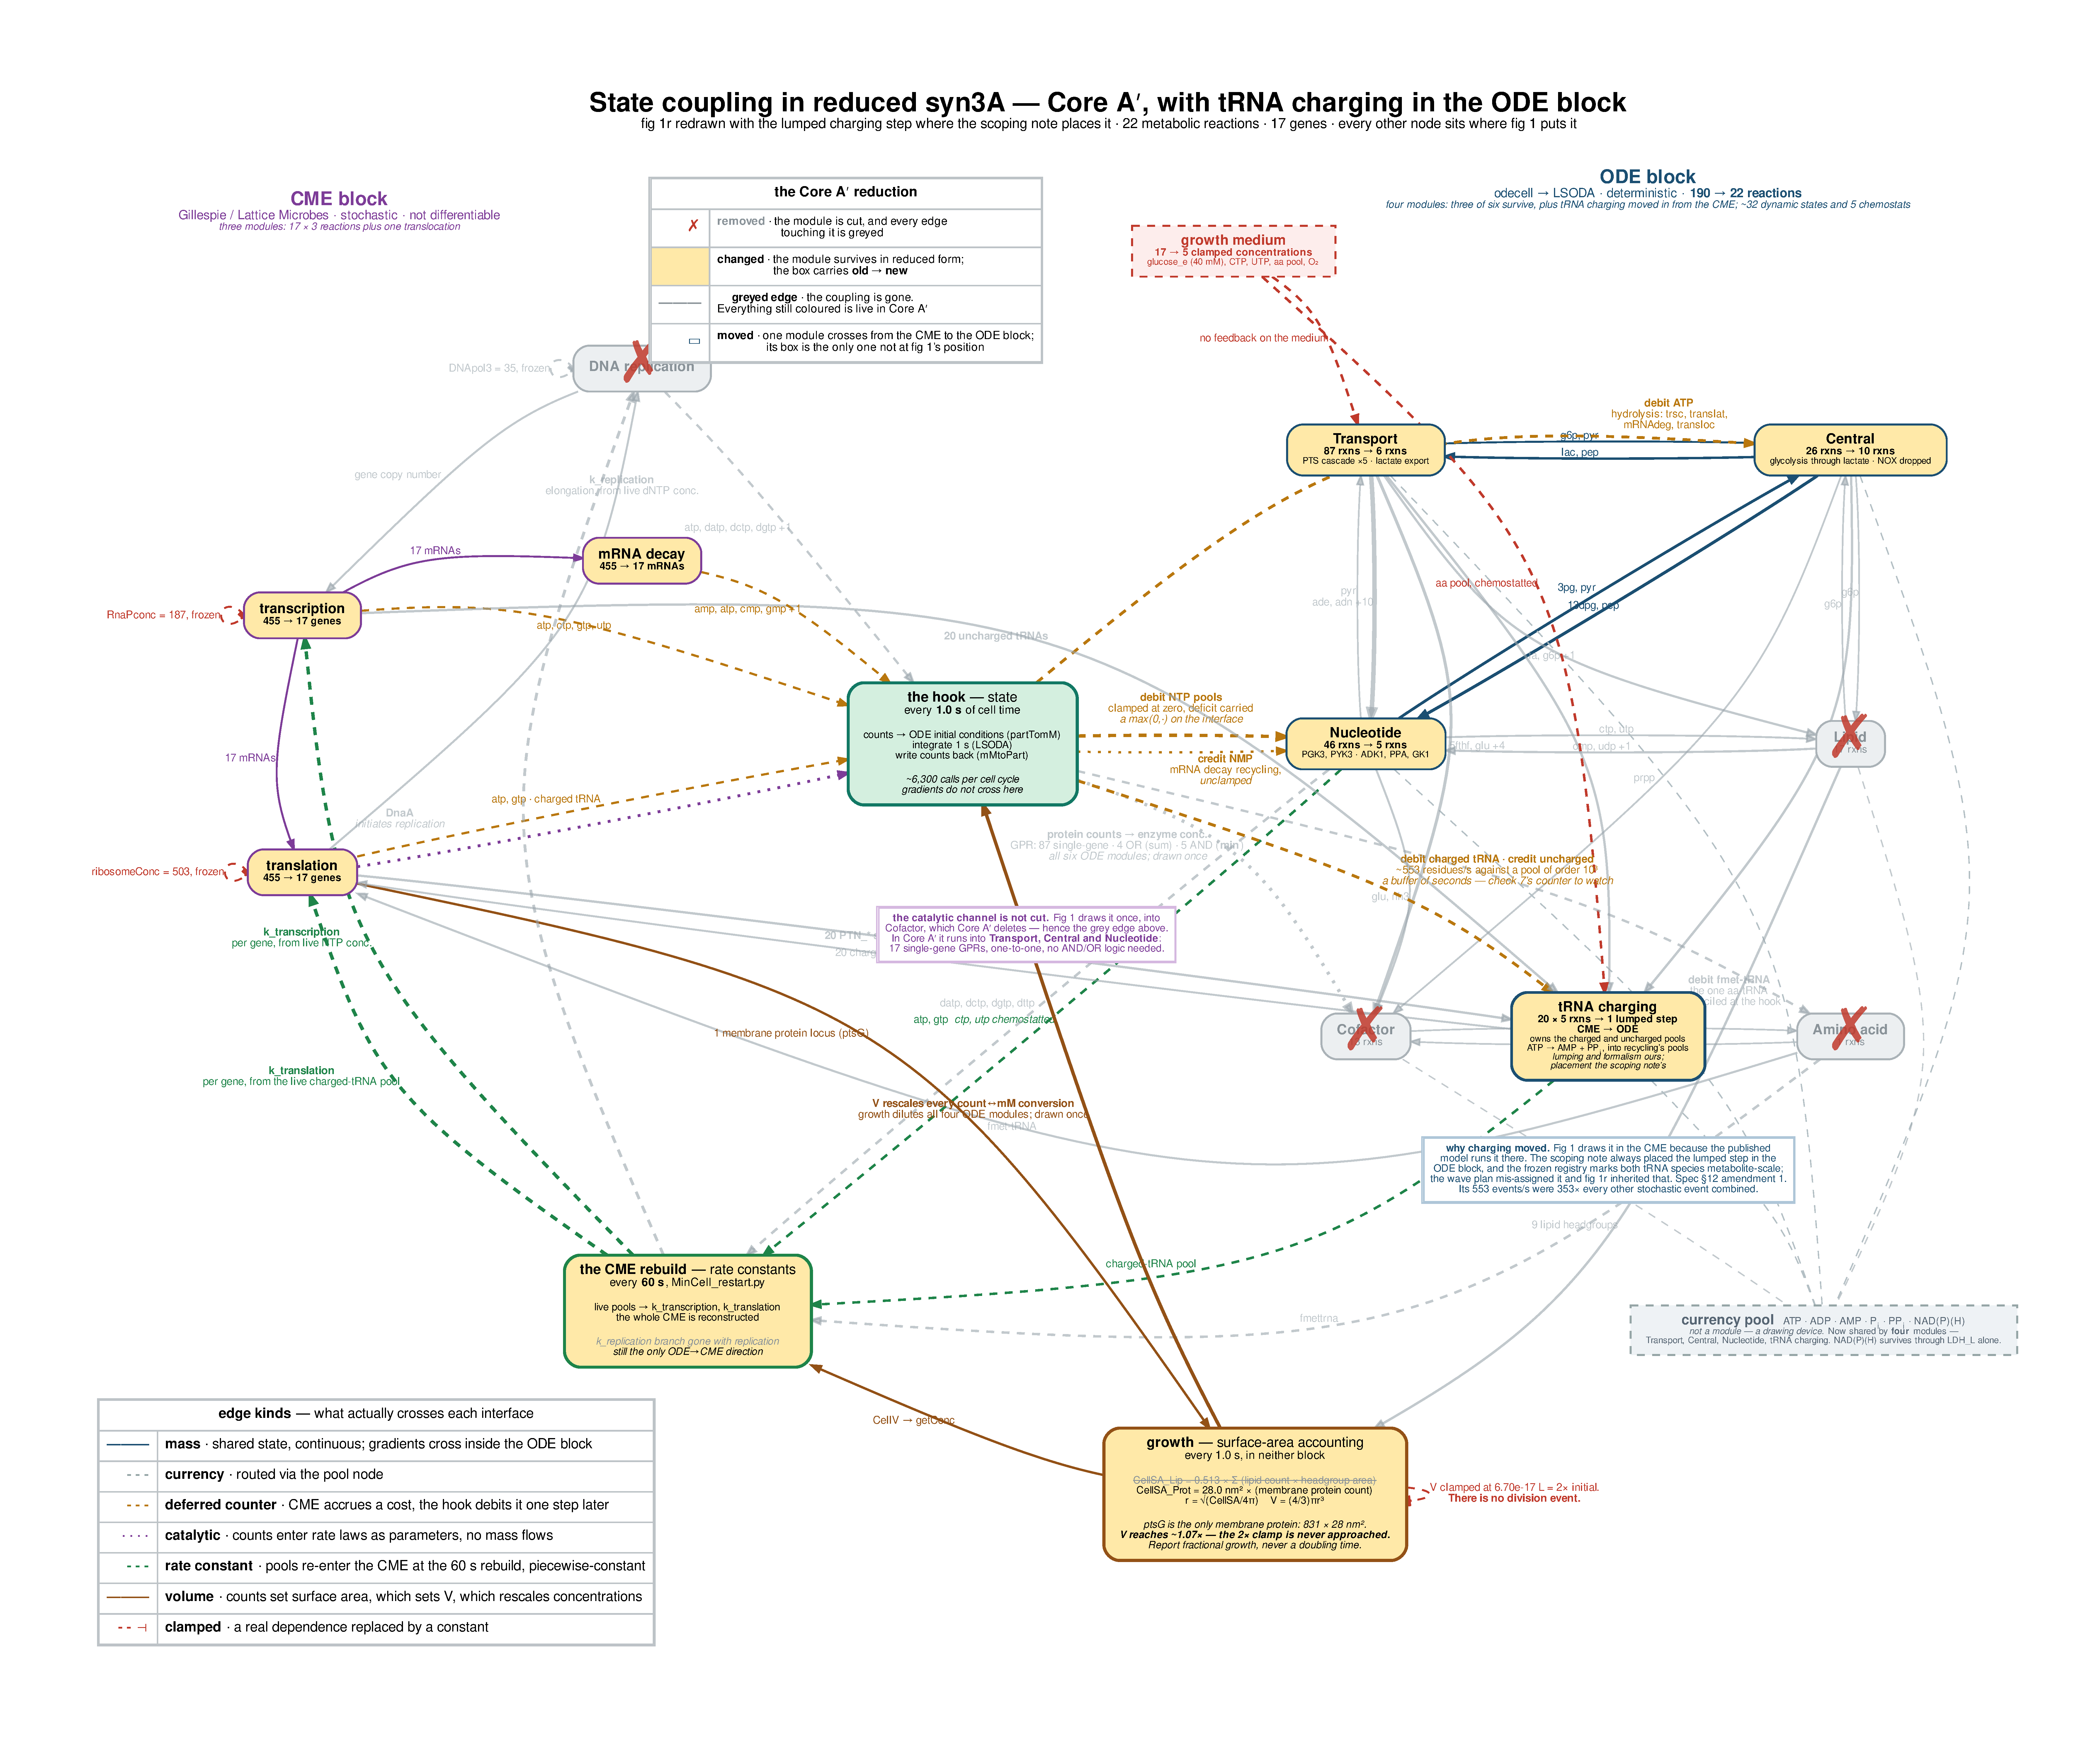
\includegraphics[width=0.85\textwidth]{fig1c_state_graph_corea.pdf}
\caption{\textbf{The reduced \syn{} model.} Metabolic modules (ODE) and
gene-expression modules (jump) and the edges between them.
\placeholder{Caption to be rewritten for the paper; the figure may need a cleaner
version for print.}}
\label{fig:model}
\end{figure*}

The model makes no claim about \syn{} itself. With most of the cell removed, it
cannot reproduce the doubling time, the metabolite levels or the proteome of the
real organism. The code refuses to report a doubling time, so that no result can
be compared with these quantities by mistake. The model's purpose is to give a
real ODE--stochastic boundary from a published whole-cell model, at a size where an
exact posterior is affordable.

\paragraph{M0, the reference system.} An exact posterior on the full reduced model
costs too much (\cref{sec:cost}). We therefore also use M0, the reduced model cut
to two genes over \pn{mzero.horizon}\,s. The two genes are GAPD, whose promoter is
the best determined, and ptsG, the membrane transporter. All metabolism stays. The
other enzyme counts are held at their measured copy numbers, and this hold is a
declared reduction. M0 has \pn{mzero.npar} free parameters: the two promoter
strengths, the transcript decay rate, the forward catalytic constants of enolase
(ENO) and aldolase (FBA), and the bulk assay noise $\sigb$.
